\chapter{\label{ch:fabrication}Experimental Details: Measurement Protocols and Device Fabrication}

\minitoc

\section{Room Temperature DC Measurements}

Describe here the probe station setup

\section{Hallbar Measurements}
Devices used for magnetometry were fabricated by Dr. Alex Gee (Fig.\ref{fig:exp:hallbar}).

\begin{figure}[hbtp]
    \begin{center}
        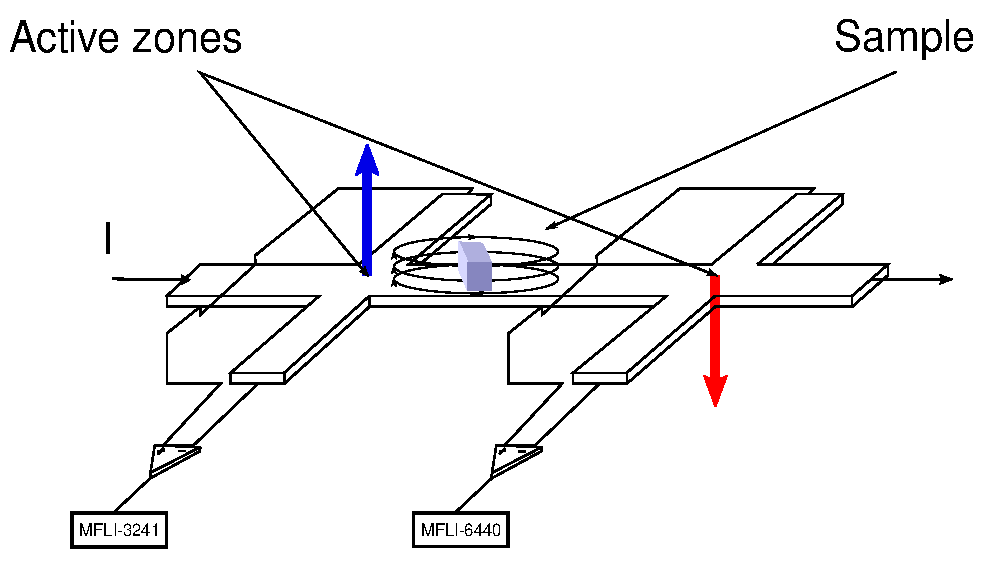
\includegraphics[width=\textwidth]{chapter_fabrication/figures/hb_sample_center.pdf}
        \caption{
            Cartoon of Hall sensors. Current flows along the central wires, while the sample sits on one of the two crosses. The sample is placed slightly offset compared to the crossposition as the magnetic field is less shielded by the gold surface. The signals are then measured in parallel by feeding first the voltage drops to two pre-amplifier and later to lock-in amplifiers.}
        \label{fig:exp:hallbar}
    \end{center}
\end{figure}

\section{Cryogenic DC Measurements}

\subsection{Temperature-dependent Protocol}
Dilution refrigerators work very well in the cryogenic temperature range but it is also possible to control the temperature thanks to the heaters. In order to measure reliably up to room temperatuer, however, one must ensures that the temperature drift is ideally slower than the time taken to acquire experimental measurements. Since there is no well-defined experimental procedure for doing so, a workaround which leverages Triton system was found and used in this thesis.

Triton heaters are capable to control the temperature precisely from base temperature ($\sim$ 25 mK) up to 30 K. In order to stabilise the temperature above this range, one has to generate a thermal link between the sample and the environment. First the heaters (mixing chamber and still, see Ch.~\ref{ch:theory}) are switched off: this enables main heat sources to be excluded from exchanging thermal energy with the sample inside the mixing chamber. Being the mixing chamber very well thermally isolated, the temperature will start raising very slowly: to give a reference number, $\sim$24h after the heaters were switched off the temperature rose by only 2 K. The pre-cooling loop is then filled with the He3/He4 mixture, creating a thermal link between the various stages within the dilution refrigerator and the mixing chamber. This results in a faster heating rate, but slow enough to allow to take quick measurements such as $I-V_\textrm{SD}$ and $I-V_\textrm{G}$ traces.

While these kind of measurements measure the current flowing through the device (after the voltage to current conversion that occurs inside the Delft box, see Ch.~\ref{ch:theory}), it is generally reccommended to acquire also the conductance. In absence of a lock-in apparatus, a possible workaround is to measure the current at various bias voltages and different gate voltage and differentiate numerically the current to obtain the conductance. In order to stabilise the temperature and remove the thermal link between the mixing chamber and the various refrigerator stages, the pre-cooling loop in then emptied, leaving the sample thermally isolated. The whole procedure was then automated in a python python script measurements, which algorithm is detailed in Alg.~\ref{alg:cap}.

\begin{algorithm}[H]
    \caption{Triton High Temperature Measurement}\label{alg:cap}
    \begin{algorithmic}[1]
        \Require Initialise Alazar, Triton and IVVI
        \Ensure Alazar, Triton, and IVVI are global
        \State Initialise Final Temperature
        \State Initialise Bias Array
        \State Initialise Target Temperatures Array
        \State Current Temperature $\gets$ Read Temperature
        \State Temperature Step $\gets$ 3
        \State Temperature Channel $\gets$ 8
        \State Precooled $\gets$ \texttt{False}
        \While{Current Temperature $<$ Final Temperature}
        \State Precooled $\gets$ \texttt{True}
        \State T $\gets$ Read Temperature
        \If{T $> 1.5$ }
        \State Temperature Channel $\gets$ 5
        \EndIf
        \For{length Bias Array}
        \State Run Gate Trace Measurement
        \EndFor
        \State T $\gets$ Read Temperature
        \If{T is in Target Temperatures Array}
        \State Precooled $\gets$ \texttt{False}
        \State Run Stability Diagram
        % \State $N \gets \frac{N}{2}$  \Comment{This is a comment}
        \EndIf
        \EndWhile
    \end{algorithmic}
\end{algorithm}

The Alazar card, Triton, and IVVI (Delft box modules) drivers are first initialised and assigned to global variables which hold their state throughout the program execution. Then several variables are initialised. The precooled variables is a routine implemented directly on top of Triton drivers which allows to set and get command directly on the instruments. While below 1 K the RuO$_2$ thermoter is used, to reliably read the temperature above this temperature one has to switch to the Cernox thermometer, hence we are setting the temperature channel variable to channel 5 within the while loop in case this conditions applies. The program then acquires gate trace and stability diagram measurements. These are functions which have been implemented and improved from scripts written by a former member of the group, Dr.\ Nicola Dotti.


\section{Cryogenic AC Measurements}

Describe here the delft box + lock-in setup and why it is so complicated to set it usepackage

\section{Thermoelectric Measurements}

Describe here the setup used for the thermoelectric devices and why it needs a dedicated section
Describe also here from a setup point of view which complications have raised during the setup (direct lines instead of dc lines,
the need to use nano-D connectors and to design the a new pcb board).


\section{General Fabrication Procedure}

The steps are well known: chip preparation, e-beam, development, metal deposition and lift-off,
graphene transfer old process, graphenea graphene

\begin{figure}[hbtp]
    \begin{center}
        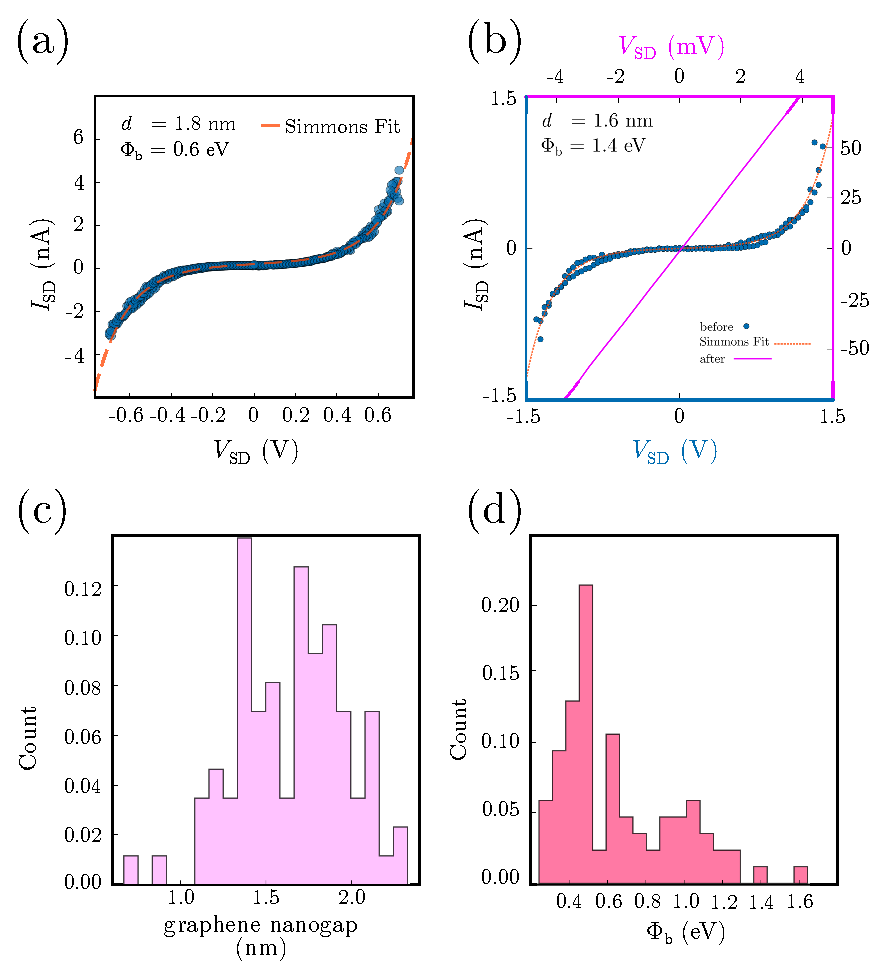
\includegraphics[width=\textwidth]{chapter_fabrication/figures/simmons.eps}
        \caption{
            Simmons Fit and fit parmaters output.}
        \label{fig:exp:simmons}
    \end{center}
\end{figure}

\subsection{Graphene Preparation and Wet Transferring}
Initially the graphene was transferred on top of the substrate through the wet transfer method. The graphene was supplied by Graphene ain 5 x 5 cm2 rectangles, with a PMMA front-layer and a back-layer
of partially removed graphene. Before transfer, the back-layer had to be fully removed via
etching, and the remaining stack appropriately sized for the substrates for this work. The
graphene arrived in a vacuum-sealed pack, which had to be transported to the cleanroom
before being opened and the following preparation steps initiated. Figure 6.2 depicts the main
stages involved in preparing the graphene for transfe

\section{Contacting Graphene Nanoribbons}

\co{Here three methods have been exploited: standard feedback electroburning, gate-dependent electroburning,
    and litographic patterning of graphene nanogaps}

The process of contacting graphene nanoribbons represents one of the major obstacles a reliable and robust fabrication. Various methodologies have been exploited in the literature. For example, litographic \gls{GNR} can be contacted through standard metal deposition techiniques by covering the substrate with a resist and evaporating metals (Pd, Au). As we have seen in the Ch.\ref{ch:introduction}, contacting bulk graphene with metals will result in Schottky barriers of various nature, which extend largely depends on the level of natural doping of graphene.

Liquid-processable \glspl{GNR} represents a further development in terms of structural integrity and shape. One of the major hurdles, however, is represented by the placement of such structures on top on a \gls{FET} geometry. In order to favour the binding interactions with the leads, we have decided to employ graphene as electrode material.

The problem of depositing graphene nanoribbons on top of graphene nanogaps could be mapped onto a well-know problem in geometric probability called Buffon's needle problem. Originally fomulated in the eighteen century, the Buffon's needle problem calculates what is the probability that by randomly throwing a needle on length $l$ the needle will cross at least a line of grid of parallel lines of width $d > l$ units apart. Several extension of this problem have been followed in the last century.

Even if the problem assumes no interactions active between the needle and the grid, the problem well capture the essence of our experiment. In the limit where the ration betwenn the needle length and the distance between the parallel lines is greater than 1, i.e. $\lambda = l/d > 1$, the probability that the needle intersects at least one line is given by \cite{uspensky1937introduction}:

\begin{equation}
    P(\lambda) =
    \begin{cases}
        \frac{2\lambda}{\pi}                                                   & \lambda\leq 1 \\
        \frac{2}{\pi}\qty(\lambda - \sqrt{\lambda^2 - 1} + \sec^{-1}(\lambda)) & \lambda>1     \\
    \end{cases}
\end{equation}

\begin{figure}[hbtp]
    \begin{center}
        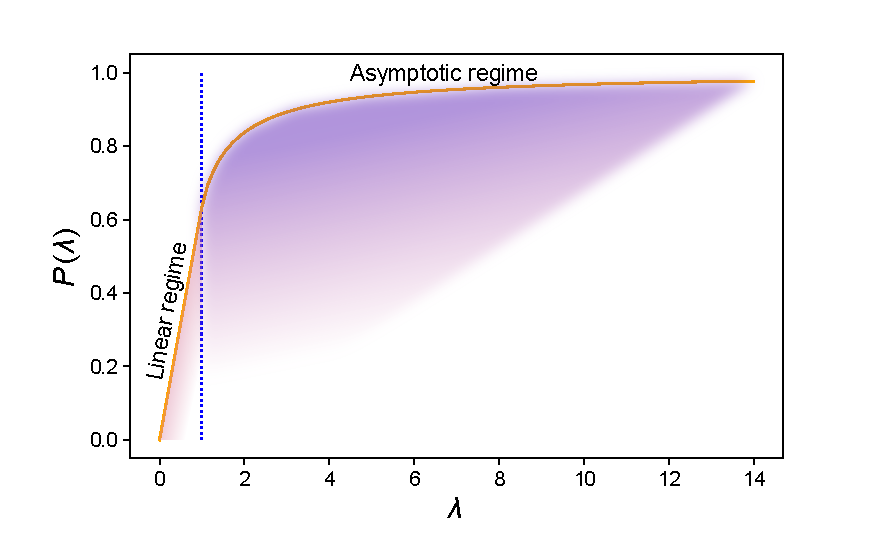
\includegraphics[width=\textwidth]{chapter_fabrication/figures/buffon_probability.pdf}
        \caption{Probability distribution as a function of the parameter $\lambda$ for a needle tossed onto a grid of equispaced parallel lines. When the needle is short ($\lambda < 1$), the coverage probability increases linearly with the length. When the needle becomes larger than the gap ($\lambda \ge 1$), the probability increases asymptotically to one and is independent of the parameter $\lambda$.}
        \label{fig:fabrication:all_transitions}
    \end{center}
\end{figure}

Fig.\ref{fig:fabrication:all_transitions} illustrates the difference between the regimes. One main assumption of this model is to completely ignore and neglect any kind of interactions between the needles.

In order to map this problem to the real-world scenario where single strand of graphene nanoribbons lay on the electrical contact, one needs to include the interaction experienced by the the ribbon and the environment when are in solution, between the ribbon and the electrical contacts and the intramolecular forces which drive a folding of a single ribbon on itself (buckle-up). In an attempt to obtaine a more realistic picture, we will briefly sketch a model that could be used by experimentalist to derive conclusion on what parameters is best to tune/change in order to obtain the higher probability to get a single \gls{GNR} briding the highest number of device per unit area.


\section{Chip Design}

Here the designs for the different chips that have been used.
Give a proper credit to Dr. Alex Gee for the fabrication of thermoelectric and the common gate ones.

\subsection{2T Design}

How convenient and 'quick' is the usage of a backgate device.
List, as usual, pro and cons

\subsection{3T Design}

Why the need to use 3T over 2T

\subsubsection{Local Gates from Waterloo}

Give proper credit

\subsubsection{Interconnected Drain and Gate}

The one I made and also made with the help of Alex

\subsection{Thermoelectric Device}

Common and different features of the thermoelectric

\section{Deposition Process and Related Phenomena}

Why it is important to study the chemistry of interfaces for
rationalising deposition processes
% Why it has been important to try different deposition techiniques
% How this has been qualitatevely addressed.
% Apolar solvents used to avoid accidental doping of the \glspl{GNR}
% Mention also the meniscus guided coating, heard in Klaus Mullen talk.
% critical speed when the crystals start to elongate in the coeating direction,
% initiating the orientation of the molecules. reducing the coating speed the domains start to decrease
% and the molecules tend to elongate better.
% transport over domains depends on the boundaries of the domains, hence the mobility goes down.
% dependence of film thickness with the v (dunno what it is, think coating speed).
